\section{Klassenbeschreibung}
\subsection{Übersicht}
Die folgende Tabelle zeigt eine Übersicht aller Klassen des Klassendiagramms gruppiert nach inhaltlichen Blöcken.

\begin{table}[htbp]
\begin{tabular}{p{5cm} c | p{5cm} c}
Frontend & Seite & Controller & Seite\\
\hline
\nameref{MainWindow} & \pageref{MainWindow} & \hyperref[entCon]{EntityController} & \pageref{entCon}\\
\nameref{DatastreamWindow} & \pageref{DatastreamWindow} & \nameref{thingCon} & \pageref{thingCon}\\
\nameref{ThingWindow} & \pageref{ThingWindow} & \nameref{dataCon} & \pageref{dataCon}\\
\nameref{SensorWindow} & \pageref{SensorWindow} & \nameref{locCon} & \pageref{locCon}\\
\nameref{LocationWindow} & \pageref{LocationWindow} & \nameref{sensCon} & \pageref{sensCon}\\
\nameref{MagicWindow} & \pageref{MagicWindow} & \nameref{ObsPCon} & \pageref{ObsPCon}\\
\nameref{PropertyWindow} & \pageref{PropertyWindow} & \nameref{ConCon} & \pageref{ConCon}\\
\  &\  & \nameref{ImpCon} & \pageref{ImpCon}\\
\  &\  & \nameref{srcCon} & \pageref{srcCon}\\
\  &\  & \nameref{htmlCon} & \pageref{htmlCon}

\end{tabular}
\end{table}

\vspace{-0.5cm}
\begin{table}[!h]
\begin{tabular}{p{5cm} c | p{5cm} c}
Entities & Seite & Datenimport & Seite\\
\hline
\hyperref[valCode]{ValueCode} & \pageref{valCode} &\nameref{uploadHandler} & \pageref{uploadHandler}\\
\hyperref[ent]{Entity} & \pageref{ent} &\hyperref[Table]{Table (Interface)} & \pageref{Table}\\
\nameref{prop} & \pageref{prop} &\hyperref[rowtable]{RowTable} & \pageref{rowtable}\\
\nameref{thing} & \pageref{thing} &\hyperref[colTable]{ColumnTable} & \pageref{colTable}\\
\nameref{data} & \pageref{data} &\hyperref[conv]{Converter (Interface)} & \pageref{conv}\\
\nameref{loc} & \pageref{loc} &\hyperref[csvConv]{CSVConverter} & \pageref{csvConv}\\
\nameref{sensor} & \pageref{sensor} &\hyperref[excelConv]{ExcelConverter} & \pageref{excelConv}\\
\nameref{oprop} & \pageref{oprop} &\nameref{obsCreator} & \pageref{obsCreator}\\
\nameref{uom} & \pageref{uom} &\nameref{dupl} & \pageref{dupl}\\
\ & \ &\nameref{timeParser} & \pageref{timeParser}\\
\ & \ &\nameref{tableParser} & \pageref{tableParser}
\end{tabular}
\end{table}

\vspace{-0.5cm}
\begin{table}[!h]
\begin{tabular}{p{5cm} c | p{5cm} c}
Konfiguration & Seite & Log- und ErrorHandling & Seite\\
\hline
\nameref{strCol} & \pageref{strCol} & \nameref{srow} & \pageref{srow}\\
\nameref{strObs} & \pageref{strObs} & \nameref{error} & \pageref{error}\\
\nameref{zoneCol} & \pageref{zoneCol} & \nameref{log} & \pageref{log}\\
\nameref{config} & \pageref{config} & \nameref{fileman} & \pageref{fileman}\\
\nameref{magic} & \pageref{magic} & \ & \ \\
\nameref{magicMap} & \pageref{magicMap} & \ & \ \\
\nameref{confman} & \pageref{confman} & \ & \ \\

\end{tabular}
\end{table}

\clearpage
\subsection{Frontend}

\begin{figure}[!h]
\centering
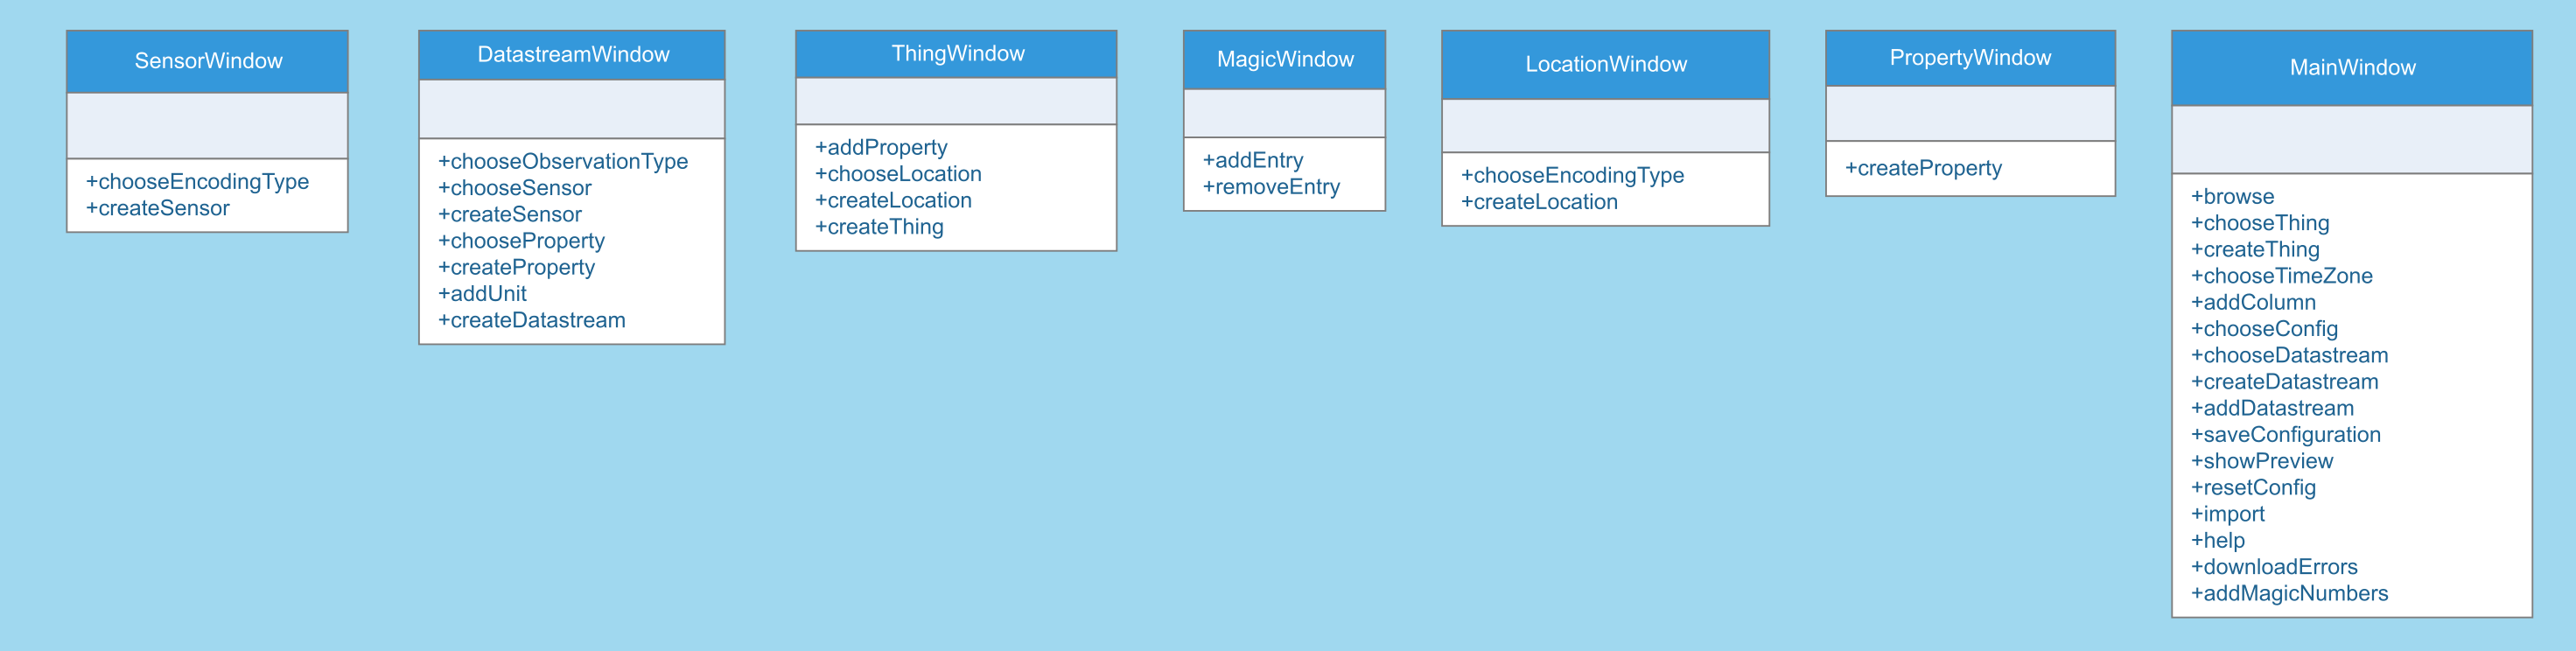
\includegraphics[scale=0.36]{uml/screenshots/frontend}
\caption{Klassen im Frontend}
\end{figure}


\subsection{MainWindow}
Diese Klasse stellt das Hauptfenster dar. 

\paragraph{Konstruktoren}
\begin{enumerate}[+]
	\item \textit{MainWindow()} Ein Konstruktor für das Hauptfenster.
\end{enumerate}

\paragraph{Methoden}

\begin{enumerate}[+]
	\item \textit{browse()} Öffnet ein Dialogfenster zum Laden einer Datei.
	\item \textit{chooseThing()} Lädt die Things in das Dropdown-Menu.
	\item \textit{createThing()} Öffnet das ThingWindow.
	\item \textit{chooseTimeZone()} Öffnet ein Fenster zum auswählen der TimeZone.
	\item \textit{addColumn()} Fügt eine Spalte für die DateTime hinzu.
	\item \textit{chooseConfig()} Füllt das Dropdown-Menu mit bis zu 20 Konfigurationen.
	\item \textit{chooseDatasteam()} Füllt das Dropdown-Menu mit den Datasteams.
	\item \textit{createDatastream()} Ruft das DatastreamWindow auf.
	\item \textit{addDatastream()} Fügt einen Datastream hinzu.
	\item \textit{saveConfiguration()} Speichert die Konfiguration.
	\item \textit{showPreview()} Zeigt eine Vorschau für den Import.
	\item \textit{resetConfig()} Setzt die bisher erstellte Konfiguration zurück.
	\item \textit{import()} Importiert die Eingabedatei in den Frostserver
	\item \textit{help()} Öffnet eine "{Help}"{-Seite}.
	\item \textit{downloadErrors()} Öffnet ein Dialogfenster um den Download der fehlgeschlagenen Zeilen zu bestätigen.
	\item \textit{addMagicNumbers()} Öffnet ein Dialogfenster um die Abbildung von Sonderzeichen zu definieren.	
\end{enumerate}



\subsection{DatastreamWindow}
Diese Klasse stellt das Fenster zum Erstellen eines Datastreams dar.

\paragraph{Konstruktoren}
\begin{enumerate}[+]
	\item \textit{DatastreamWindow()} Ein Konstruktor für das Fenster.
\end{enumerate}

\paragraph{Methoden}

\begin{enumerate}[+]
	\item \textit{chooseObservationType()} Füllt das zugehörige Dropdown-Menu mit den Observation-Types.
	\item \textit{chooseSensor()} Füllt das Dropdown-Menu zur Auswahl eines Sensors mit Daten.
	\item \textit{createSensor()} Öffnet das Fenster zum Erstellen eines Sensors.
	\item \textit{chooseProperty()} Füllt das Dropdown-Menu mit Daten.
	\item \textit{createProperty()} Öffnet das Fenster zum Erstellen einer Property.
	\item \textit{addUnit()} Fügt eine Reihe für ein neues Unit hinzu.
	\item \textit{createDatastream()} Erstellt mit den eingegebenen Daten einen neuen Datastream.
\end{enumerate}



\subsection{ThingWindow}
Diese Klasse stellt das Fenster zum Erstellen eines Things dar.

\paragraph{Konstruktoren}
\begin{enumerate}[+]
	\item \textit{ThingWindow()} Ein Konstruktor für das Fenster.
\end{enumerate}

\paragraph{Methoden}

\begin{enumerate}[+]
	\item \textit{addProperty()} Fügt eine Reihe für eine weitere Property hinzu.
	\item \textit{chooseLocation()} Füllt das Dropdown-Menu mit Locations. 
	\item \textit{createLocation()} Öffnet das Fenster LocationWindow.
	\item \textit{createThing()} Erstellt aus den gegebenen Daten ein Thing.
\end{enumerate}



\subsection{SensorWindow}
Diese Klasse stellt das Fenster zum Erstellen eines Sensors dar.

\paragraph{Konstruktoren}
\begin{enumerate}[+]
	\item \textit{SensorWindow()} Ein Konstruktor für das Fenster.
\end{enumerate}

\paragraph{Methoden}

\begin{enumerate}[+]
	\item \textit{chooseEncodingType()} Füllt das dazugehörige Dropdown-Menu mit den Encodingtypes.
	\item \textit{createSensor()} Erstellt aus den gegebenen Daten ein Sensor-Objekt.
		
\end{enumerate}



\subsection{LocationWindow}
Diese Klasse stellt das Fenster zum Erstellen einer Location dar.

\paragraph{Konstruktoren}
\begin{enumerate}[+]
	\item \textit{LocationWindow()} Ein Konstruktor für das Fenster.
\end{enumerate}

\paragraph{Methoden}

\begin{enumerate}[+]
	\item \textit{chooseEncodingType()} Füllt das dazugehörige Dropdown-Menu mit den Encodingtypes.
	\item \textit{createLocation()} Erstellt aus den gegebenen Daten ein Location-Objekt.
	
\end{enumerate}




\subsection{MagicWindow}
Diese Klasse stellt das Fenster zum Erstellen der Sonderzeichen-Abbildungen dar.

\paragraph{Konstruktoren}
\begin{enumerate}[+]
	\item \textit{MagicWindow()} Ein Konstruktor für das Fenster.
\end{enumerate}

\paragraph{Methoden}

\begin{enumerate}[+]
	\item \textit{addEntry()} Fügt eine Abbildung hinzu.
	\item \textit{createMagic()} Erstellt aus den gegebenen Daten ein MagicNumbers-Objekt.	
\end{enumerate}



\subsection{PropertyWindow}
Diese Klasse stellt das Fenster zum Erstellen einer Property dar.

\paragraph{Konstruktoren}
\begin{enumerate}[+]
	\item \textit{PropertyWindow()} Ein Konstruktor für das Fenster.
\end{enumerate}

\paragraph{Methoden}

\begin{enumerate}[+]
	\item \textit{createProperty()} Erstellt aus den gegebenen Daten ein 	Property-Objekt.	
\end{enumerate}




\clearpage
\subsection{Controller}
\begin{figure}[!h]
\centering
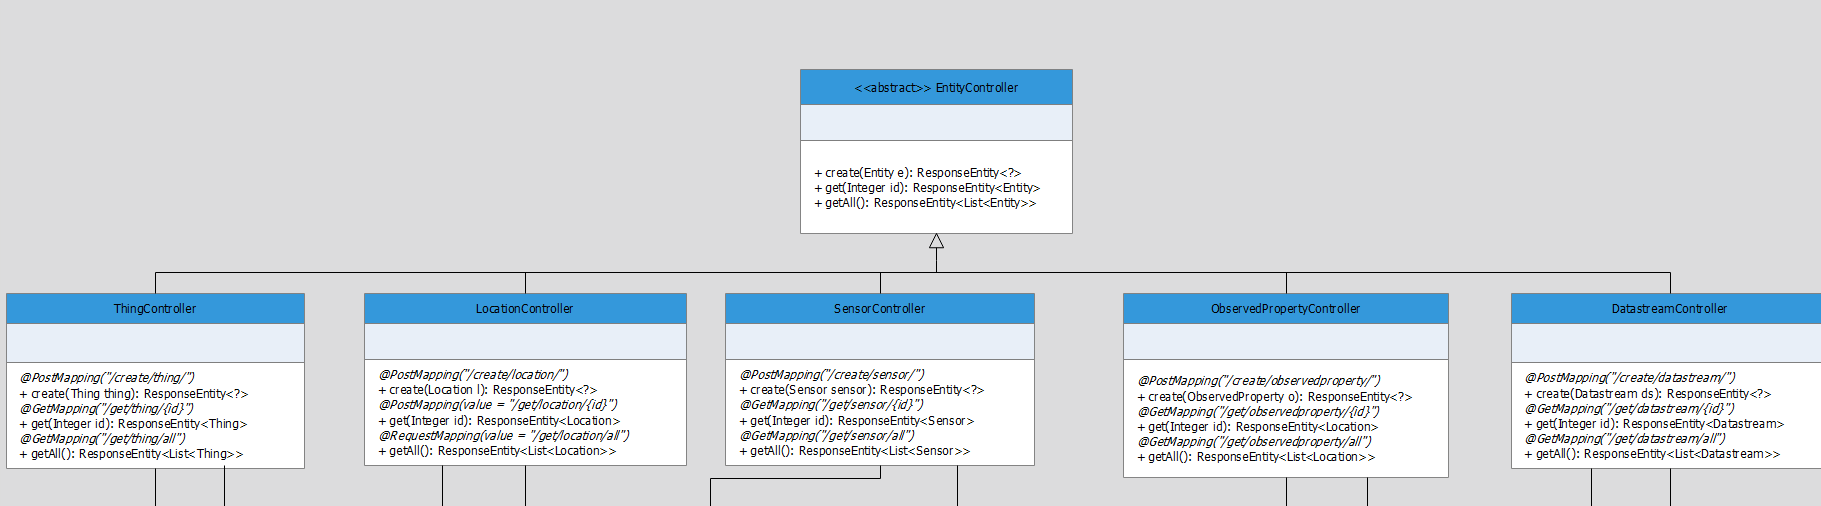
\includegraphics[scale=0.365]{uml/screenshots/entity-controller}
\caption{Entity-Controller}
\end{figure}
\begin{figure}[!h]
\centering
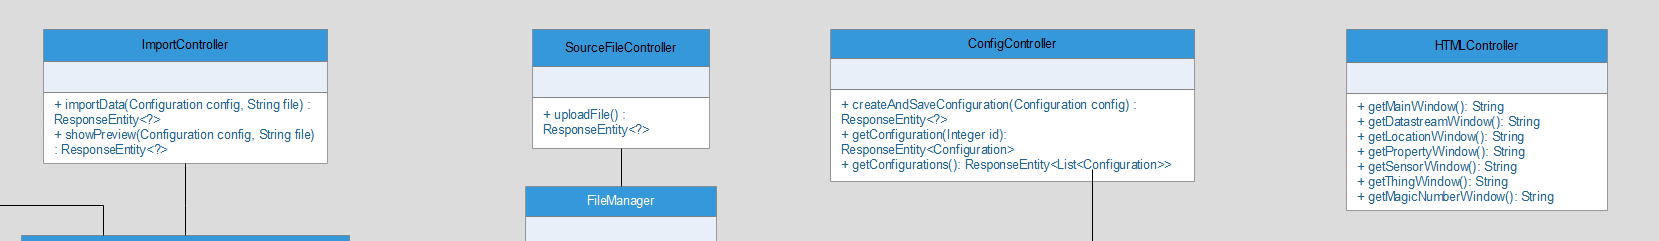
\includegraphics[scale=0.4]{uml/screenshots/controller}
\caption{Restliche Controller}
\end{figure}


\subsection*{<<abstract>> EntityController}\label{entCon}
Diese Controller-Klasse empfängt Anfragen vom Frontend, die das Erstellen oder Abrufen von Entitäten betreffen.

\paragraph{Methoden}

\begin{enumerate}[+]
	\item \textit{ create(Entity e): ResponseEntity<?> }\\
	erstellt eine neue Entity und lädt diese auf den FROST-Server
	
		\begin{enumerate}[$\bullet$]
			\item \textit{Entity e} die Entität, die erstellt werden soll

		\end{enumerate}
		\vspace{-0.2cm}
		\begin{enumerate}[$\circ$]
			\item \textit{ResponseEntity<?>} Rückgabe-Typ von Controller-Klassen
		\end{enumerate}
	
	\item \textit{ get(int id): ResponseEntity<Entity> }\\
	sucht auf dem Server die Entität mit der angegebenen id und gibt sie zurück (NULL im Fehlerfall)
	
		\begin{enumerate}[$\bullet$]
			\item \textit{int id} ID der Entität, die geladen werden soll
		
		\end{enumerate}
		\vspace{-0.2cm}
		\begin{enumerate}[$\circ$]
			\item \textit{ResponseEntity<Entity>} Entität mit angegebener ID (Rückgabe-Typ von Controller-Klassen)
		\end{enumerate}
	\item \textit{ getAll(): ResponseEntity<List<Entity>> }\\
	gibt alle auf dem FROST-Server gespeicherten Entitäten zurück
	
	\begin{enumerate}[$\circ$]
		\item \textit{ResponseEntity<List<Entity>>} alle Entitäten auf dem FROST-Server (Rückgabe-Typ von Controller-Klassen)
	\end{enumerate}


\end{enumerate}	

\clearpage
\subsection{ThingController}

\paragraph{Beschreibung}
Diese Controller-Klasse empfängt Anfragen vom Frontend, die das Erstellen oder Abrufen von Things betreffen. Zur Bearbeitung dieser Anfragen greift die Klasse auf den Frost-Client zu.


\paragraph{Attribute}

\paragraph{Methoden}
\begin{itemize}
\item[+] \textit{ createThing(String name, String description, Map<String, Object> properties, Location location) : void }
erstellt mithilfe des Frost-Client ein neues Thing und lädt es auf den Frostserver.
\item[+] \textit{getThing(int id) : Thing}
sucht auf dem Server das Thing mit der angegebenen id und gibt es zurück (NULL im Fehlerfall)
\item[+] \textit{getThings(String begin) : List<Thing> }
sucht auf dem Frost-Server die Things (maximal die ersten 7), deren Namen mit der angegeben Zeichenkette beginnen.
\end{itemize}
\clearpage
\subsection{DatastreamController}

\paragraph{Beschreibung}
Diese Controller-Klasse empfängt Anfragen vom Frontend, die das Erstellen oder Abrufen von (Multi-)Datastreams betreffen. Zur Bearbeitung dieser Anfragen greift die Klasse auf den Frost-Client zu.


\paragraph{Attribute}

\paragraph{Methoden}
\begin{itemize}
\item[+] \textit{create(Datastream ds): ResponseEntity<?> }
erstellt mithilfe des Frost-Client einen neuen (Multi-)Datastream und lädt diesen auf den Frostserver
\item[+] \textit{get(int id) : ResponseEntity<Datastream>}
sucht auf dem Server den (Multi-)Datastream mit der angegebenen id und gibt diesen zurück (NULL im Fehlerfall)
\item[+] \textit{getAll(): ResponseEntity<List<Datastream>> }
gibt alle auf dem FROST-Server gespeicherten (Multi-)Datastreams zurück
\end{itemize}
\clearpage
\subsection*{LocationController}\label{locCon}
Diese Controller-Klasse empfängt Anfragen vom Frontend, die das Erstellen oder Abrufen von Locations betreffen.

\paragraph{Methoden}

\begin{enumerate}[+]
	\item \textit{ create(Location loc): ResponseEntity<?> }\\
	erstellt eine neue Location und lädt diese auf den FROST-Server
	
	\begin{enumerate}[$\bullet$]
		\item \textit{Location loc} die Location, die erstellt werden soll
		
	\end{enumerate}
	\vspace{-0.2cm}
	\begin{enumerate}[$\circ$]
		\item \textit{ResponseEntity<?>} Rückgabe-Typ von Controller-Klassen
	\end{enumerate}
	
	\item \textit{ get(int id): ResponseEntity<Location> }\\
	sucht auf dem Server die Location mit der angegebenen id und gibt sie zurück (NULL im Fehlerfall)
	
	\begin{enumerate}[$\bullet$]
		\item \textit{int id} ID der Location, die geladen werden soll
		
	\end{enumerate}
	\vspace{-0.2cm}
	\begin{enumerate}[$\circ$]
		\item \textit{ResponseEntity<Location>} Location mit angegebener ID (Rückgabe-Typ von Controller-Klassen)
	\end{enumerate}
	\item \textit{ getAll(): ResponseEntity<List<Location>> }\\
	gibt alle auf dem FROST-Server gespeicherten Locations zurück
	
	\begin{enumerate}[$\circ$]
		\item \textit{ResponseEntity<List<Location>>} alle Locations auf dem FROST-Server (Rückgabe-Typ von Controller-Klassen)
	\end{enumerate}
	
	
\end{enumerate}	
\clearpage
\subsection*{SensorController}\label{sensCon}
Diese Controller-Klasse empfängt Anfragen vom Frontend, die das Erstellen oder Abrufen von Sensoren betreffen.

\paragraph{Methoden}

\begin{enumerate}[+]
	\item \textit{ create(Sensor sensor): ResponseEntity<?> }\\
	erstellt einen neuen Sensor und lädt ihn auf den FROST-Server
	
	\begin{enumerate}[$\bullet$]
		\item \textit{Sensor sensor} der Sensor, der erstellt werden soll
		
	\end{enumerate}
	\vspace{-0.2cm}
	\begin{enumerate}[$\circ$]
		\item \textit{ResponseEntity<?>} Rückgabe-Typ von Controller-Klassen
	\end{enumerate}
	
	\item \textit{ get(Integer id): ResponseEntity<Sensor> }\\
	sucht auf dem Server den Sensor mit der angegebenen id und gibt ihn zurück (NULL im Fehlerfall)
	
	\begin{enumerate}[$\bullet$]
		\item \textit{Integer id} ID des Sensors, der geladen werden soll
		
	\end{enumerate}
	\vspace{-0.2cm}
	\begin{enumerate}[$\circ$]
		\item \textit{ResponseEntity<Sensor>} Sensor mit angegebener ID (Rückgabe-Typ von Controller-Klassen)
	\end{enumerate}
	\item \textit{ getAll(): ResponseEntity<List<Sensor>> }\\
	gibt alle auf dem FROST-Server gespeicherten Sensoren zurück
	
	\begin{enumerate}[$\circ$]
		\item \textit{ResponseEntity<List<Sensor>>} alle Sensoren auf dem FROST-Server (Rückgabe-Typ von Controller-Klassen)
	\end{enumerate}
	
	
\end{enumerate}
\clearpage
\subsection*{ObservedPropertyController}\label{ObsPCon}
Diese Controller-Klasse empfängt Anfragen vom Frontend, die das Erstellen oder Abrufen von ObservedProperties betreffen.

\paragraph{Methoden}

\begin{enumerate}[+]
	\item \textit{ create(ObservedProperty op): ResponseEntity<?> }\\
	erstellt eine neue ObservedProperty und lädt diese auf den FROST-Server
	
	\begin{enumerate}[$\bullet$]
		\item \textit{ObservedProperty op} die ObservedProperty, die erstellt werden soll
		
	\end{enumerate}
	\vspace{-0.2cm}
	\begin{enumerate}[$\circ$]
		\item \textit{ResponseEntity<?>} Rückgabe-Typ von Controller-Klassen
	\end{enumerate}
	
	\item \textit{ get(Integer id): ResponseEntity<ObservedProperty> }\\
	sucht auf dem Server die ObservedProperty mit der angegebenen id und gibt sie zurück (NULL im Fehlerfall)
	
	\begin{enumerate}[$\bullet$]
		\item \textit{Integer id} ID der ObservedProperty, die geladen werden soll
		
	\end{enumerate}
	\vspace{-0.2cm}
	\begin{enumerate}[$\circ$]
		\item \textit{ResponseEntity<ObservedProperty>} ObservedProperty mit angegebener ID (Rückgabe-Typ von Controller-Klassen)
	\end{enumerate}
	\item \textit{ getAll(): ResponseEntity<List<ObservedProperty>> }\\
	gibt alle auf dem FROST-Server gespeicherten ObservedProperties zurück
	
	\begin{enumerate}[$\circ$]
		\item \textit{ResponseEntity<List<ObservedProperty>>} alle ObservedProperties auf dem FROST-Server (Rückgabe-Typ von Controller-Klassen)
	\end{enumerate}
	
	
\end{enumerate}	
\clearpage

\subsection{ConfigurationController}

\paragraph{Beschreibung}
Diese Controller-Klasse empfängt Anfragen vom Frontend, die das Erstellen oder Abrufen von Konfigurationen betreffen. Zur Bearbeitung dieser Anfragen greift die Klasse auf den ConfigurationManager zu.


\paragraph{Attribute}
\begin{itemize}
\item[-] \textit{int configCounter} zählt die Anzahl gespeicherter Configurations
\end{itemize}

\paragraph{Methoden}
\begin{itemize}
\item[+] \textit{ createAndSaveConfiguration(Configuration config) : ResponseEntity<?> }
erstellt mithilfe des ConfigurationManagers eine neue Configuration, speichert sie ab und erhöht der configCounter
\item[+] \textit{getConfiguration(int id) : ResponseEntity<Configuration>}
sucht auf dem Server das Thing mit der angegebenen id und gibt es zurück (NULL im Fehlerfall)
\item[+] \textit{getConfigurations() : ResponseEntity<List<Configuration>> }
sucht aus dem Speicher alle Configurations und gibt sie zurück
\end{itemize}
\clearpage
\subsection{ImportController}

\paragraph{Beschreibung}
Diese Controller-Klasse empfängt Anfragen vom Frontend, die den Daten-Import oder die Vorschau betreffen.


\paragraph{Attribute}

\paragraph{Methoden}
\begin{itemize}
\item[+] \textit{ importData(Configuration config, String file) : ResponseEntity<?>}
 erstellt eine aktuelle Configuration Instanz, die daraufhin vom Uploader abgerufen wird um den Daten-Import durchzuführen
\item[+] \textit{showPreview(Configuration config, String file) : ResponseEntity<?>}
erstellt eine aktuelle Configuration Instanz, die daraufhin vom Uploader abgerufen wird um eine Vorschau anzuzeigen
\end{itemize}
\clearpage
\subsection{SourceFileController}

\paragraph{Beschreibung}
Diese Controller-Klasse lädt die Quelldatei (sobald sie ausgewählt wurde) ins Backend.


\paragraph{Attribute}

\paragraph{Methoden}
\begin{itemize}
\item[+] \textit{ uploadFile() : ResponseEntity<?>}
 lädt die Quelldatei mithilfe des FileManagers ins Backend 
\end{itemize}
\clearpage
\subsection*{HTMLController}\label{htmlCon}
Diese Controller-Klasse regelt die Darstellung der HTML-Seiten.


\paragraph{Methoden}
\begin{itemize}
	\item[+] \textit{ getMainWindow(): String } \\
	Gibt die HTML-Datei zurück, die das Hauptfenster darstellt
	\begin{enumerate}[$\circ$]
		\item \textit{String}: Der Name der HTML-Datei
	\end{enumerate}

	\item[+] \textit{ getDatastreamWindow(): String } \\
	Gibt die HTML-Datei zurück, die das Popup zum Erstellen eines neuen (Multi)Datastreams darstellt
	\begin{enumerate}[$\circ$]
		\item \textit{String}: Der Name der HTML-Datei
	\end{enumerate}

	\item[+] \textit{ getLocationWindow(): String } \\
	Gibt die HTML-Datei zurück, die das Location-Erstellen-Popup darstellt
	\begin{enumerate}[$\circ$]
		\item \textit{String}: Der Name der HTML-Datei
	\end{enumerate}

	\item[+] \textit{ getPropertyWindow(): String } \\
	Gibt die HTML-Datei zurück, die das Property-Popup darstellt
	\begin{enumerate}[$\circ$]
		\item \textit{String}: Der Name der HTML-Datei
	\end{enumerate}

	\item[+] \textit{ getSensorWindow(): String } \\
	Gibt die HTML-Datei zurück, die das Sensor-Popup darstellt
	\begin{enumerate}[$\circ$]
		\item \textit{String}: Der Name der HTML-Datei
	\end{enumerate}

	\item[+] \textit{ getThingWindow(): String } \\
	Gibt die HTML-Datei zurück, die das Thing-Erstellen-Popup darstellt
	\begin{enumerate}[$\circ$]
		\item \textit{String}: Der Name der HTML-Datei
	\end{enumerate}

	\item[+] \textit{ getMagicNumberWindow(): String } \\
	Gibt die HTML-Datei zurück, die das Popup darstellt, mit dem die Magic Numbers bearbeitet werden können
	\begin{enumerate}[$\circ$]
		\item \textit{String}: Der Name der HTML-Datei
	\end{enumerate}
\end{itemize}

\clearpage
\subsection{Entities}
\begin{figure}[!h]
\centering
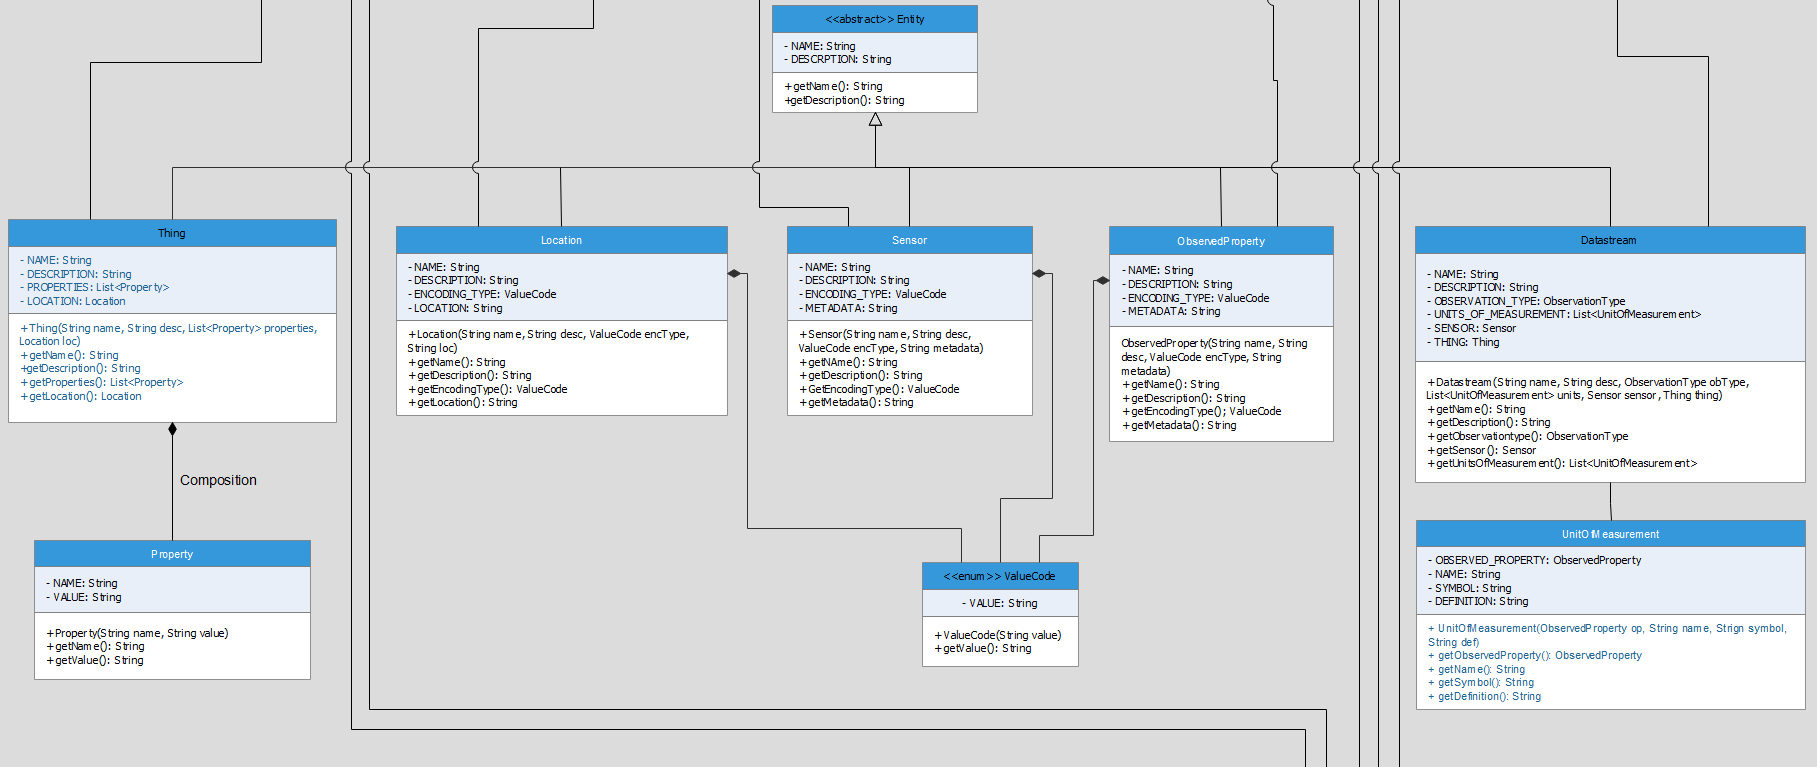
\includegraphics[scale=0.36]{uml/screenshots/entity}
\caption{Entity-Klassen}
\end{figure}
\subsection{<{<{enum}>}> ValueCode}
Stellt ValueCodes bereit

\paragraph{Attribute}
\begin{enumerate}[$\bullet$]
	\item \textit{VALUE : String} Wert des ValueCodes
\end{enumerate}

\paragraph{Konstruktoren}
\begin{enumerate}[+]
	\item \textit{ ValueCode(String value)}
	erstellt eine neue ValueCode-Instanz
	\begin{enumerate}[$\bullet$]
		\item \textit{String value} Wert des ValueCodes

	\end{enumerate}
	
\end{enumerate}

\subsection{<{<{abstract}>}> Entity}
Diese Klasse Beschreibt eine abstrakte Entität 

\paragraph{Attribute}
\begin{enumerate}[$\bullet$]
	\item \textit{NAME : String} Name der Entität
	\item \textit{DESCRIPTION : String} Beschreibung der Entität
\end{enumerate}


\clearpage
\subsection{Property}
Diese Klasse Beschreibt eine Property, eine Eigenschaft eines Things.

\paragraph{Attribute}
\begin{enumerate}[$\bullet$]
	\item \textit{NAME : String} Name der Eigenschaft
	\item \textit{VALUE : String} Wert der Eigenschaft
\end{enumerate}

\paragraph{Konstruktoren}
\begin{enumerate}[+]
	\item \textit{ Property(String name, String value)}
	erstellt eine neue Property-Instanz
	\begin{enumerate}[$\bullet$]
		\item \textit{String name} Name der Eigenschaft
		\item \textit{String value} Wert der Eigenschaft
	\end{enumerate}
	
\end{enumerate}

\clearpage
\subsection{Thing}
Diese Klasse Beschreibt ein Thing (deutsch: Gegenstand/Ding), ein Objekt der physischen oder virtuellen Welt.

\paragraph{Attribute}
\begin{enumerate}[$\bullet$]
	\item \textit{NAME : String} Name des Things
	\item \textit{DESCRIPTION : String} Beschreibung des Things
	\item \textit{PROPERTIES : List<Property>} Eigenschaften des Things
	\item \textit{LOCATION : Location} Ort an dem sich das Thing befindet
\end{enumerate}

\paragraph{Konstruktoren}
\begin{enumerate}[+]
	\item \textit{Thing(String name, String desc, List<Property> properties, Location loc)}
	erstellt eine neue Thing-Instanz
	\begin{enumerate}[$\bullet$]
		\item \textit{String name} Name des Things
		\item \textit{String desc} Beschreibung des Things
		\item \textit{List<Property> properties} Eigenschaften des Things
		\item \textit{Location loc} Ort an dem sich das Thing befindet
	\end{enumerate}
	
\end{enumerate}

\clearpage
\subsection{Datastream}
Diese Klasse Beschreibt einen (Multi-)Datastream. Ein Datastream ist eine fortlaufende Sammlung von Messungen (Observations) des selben Sensors und der selben ObservedProperty. Multi-Datastreams haben mehrere ObservedProperties.

\paragraph{Attribute}
\begin{enumerate}[$\bullet$]
	\item \textit{NAME : String} Name des Datastreams
	\item \textit{DESCRIPTION : String} Beschreibung des Datastreams
	\item \textit{OBSERVATION\_TYPE: ObservationType} Beobachtungs-Typ des Datastreams
	\item \textit{UNITS\_OF\_MEASUREMENT: List<UnitOfMeasurement>} Maßeinheit(en) des Datastreams: eine bei Datastream, mehrere bei MultiDatastream
	\item \textit{SENSOR: Sensor} Sensor des Datastreams
	\item \textit{THING: Thing} Thing des Datastreams
	
\end{enumerate}

\paragraph{Konstruktoren}
\begin{enumerate}[+]
	\item \textit{Datastream(String name, String desc, ObservationType obType,  List<UnitOfMeasurement> units, Sensor sensor, Thing thing)}
	erstellt eine neue Thing-Instanz
	\begin{enumerate}[$\bullet$]
		\item \textit{String name} Name des Datastreams
		\item \textit{String desc} Beschreibung des Datastreams
		\item \textit{ObservationType obType} Beobachtungs-Typ des Datastreams
		\item \textit{List<UnitOfMeasurement> units} Maßeinheit(en) des Datastreams: eine bei Datastream, mehrere bei MultiDatastream
		\item \textit{Sensor sensor} Sensor des Datastreams
		\item \textit{Thing thing} Thing des Datastreams
	\end{enumerate}
	
\end{enumerate}

\clearpage
\subsection{Location}
Diese Klasse Beschreibt eine Location, den Ort eines oder mehrerer Things.

\paragraph{Attribute}
\begin{enumerate}[$\bullet$]
	\item \textit{NAME : String} Name der Location
	\item \textit{DESCRIPTION : String} Beschreibung der Location
	\item \textit{ENCODING\_TYPE: ValueCode} Kodierung der Location
	\item \textit{LOCATION: String} Textuelle Darstellung des Ortes
\end{enumerate}

\paragraph{Konstruktoren}
\begin{enumerate}[+]
	\item \textit{ Location(String name, String desc, ValueCode encType, String loc)}
	erstellt eine neue Location-Instanz
	\begin{enumerate}[$\bullet$]
		\item \textit{String name} Name der Location
		\item \textit{String desc} Beschreibung der Location
		\item \textit{ValueCode encType} Kodierung der Location
		\item \textit{String loc} Textuelle Darstellung des Ortes
	\end{enumerate}
	
\end{enumerate}

\clearpage
\subsection*{Sensor}\label{sensor}
Diese Klasse Beschreibt einen Sensor. Ein Sensor misst eine Eigenschaft um eine Approximation des Wertes der Eigenschaft zurückzugeben.
\paragraph{Attribute}
\begin{enumerate}[$\bullet$]
	\item \textit{NAME : String} Name des Sensors
	\item \textit{DESCRIPTION : String} Beschreibung des Sensors
	\item \textit{ENCODING\_TYPE: ValueCode} Kodierung des Sensors
	\item \textit{METADATA: String} Metadaten des Sensors
\end{enumerate}

\paragraph{Konstruktoren}
\begin{enumerate}[+]
	\item \textit{ Sensor(String name, String desc, ValueCode encType, String metadata)}
	erstellt eine neue Sensor-Instanz
	\begin{enumerate}[$\bullet$]
		\item \textit{String name} Name des Sensors
		\item \textit{String description} Beschreibung des Sensors
		\item \textit{ValueCode encType} Kodierung des Sensors
		\item \textit{String metadata} Metadaten des Sensors
	\end{enumerate}
	
\end{enumerate}

\clearpage
\subsection{ObservedProperty}
Diese Klasse Beschreibt eine ObservedProperty (deutsch: beobachtete Eigenschaft). Sie spezifiziert das Phänomen einer Beobachtung (Observation).

\paragraph{Attribute}
\begin{enumerate}[$\bullet$]
	\item \textit{NAME : String} Name der ObservedProperty
	\item \textit{DESCRIPTION : String} Beschreibung der ObservedProperty
	\item \textit{ENCODING\_TYPE: ValueCode} Kodierung der ObservedProperty
	\item \textit{METADATA: String} Metadaten der ObservedProperty
\end{enumerate}

\paragraph{Konstruktoren}
\begin{enumerate}[+]
	\item \textit{ ObservedProperty(String name, String desc, ValueCode encType, String metadata)}
	erstellt eine neue Location-Instanz
	\begin{enumerate}[$\bullet$]
		\item \textit{String name} Name der ObservedProperty
		\item \textit{String desc} Beschreibung der ObservedProperty
		\item \textit{ValueCode encType} Kodierung der ObservedProperty
		\item \textit{String metadata} Metadaten der ObservedProperty
	\end{enumerate}
	
\end{enumerate}

\clearpage
\subsection{UnitOfMeasurement}
Beschreibt eine Maßeinheit.

\paragraph{Attribute}
\begin{enumerate}[$\bullet$]
	\item \textit{NAME : String} Name der Einheit
	\item \textit{SYMBOL : String} Symbol der Einheit
	\item \textit{DEFINITION: String} Definition der Einheit
	\item \textit{OBSERVED\_PROPERTY: ObservedProperty} Beobachtete Eigenschaft der Einheit
\end{enumerate}

\paragraph{Konstruktoren}
\begin{enumerate}[+]
	\item \textit{ UnitOfMeasurement(String name, String symbol, String def, ObservedProperty op)}
	erstellt eine neue UnitOfMeasurement-Instanz
	\begin{enumerate}[$\bullet$]
		\item \textit{String name} Name der Einheit
		\item \textit{String symbol} Symbol der Einheit
		\item \textit{String def} Definition der Einheit
		\item \textit{ObservedProperty op} Beobachtete Eigenschaft der Einheit
	\end{enumerate}
	
\end{enumerate}


\clearpage
\subsection{Datenimport}
\begin{figure}[!h]
\centering
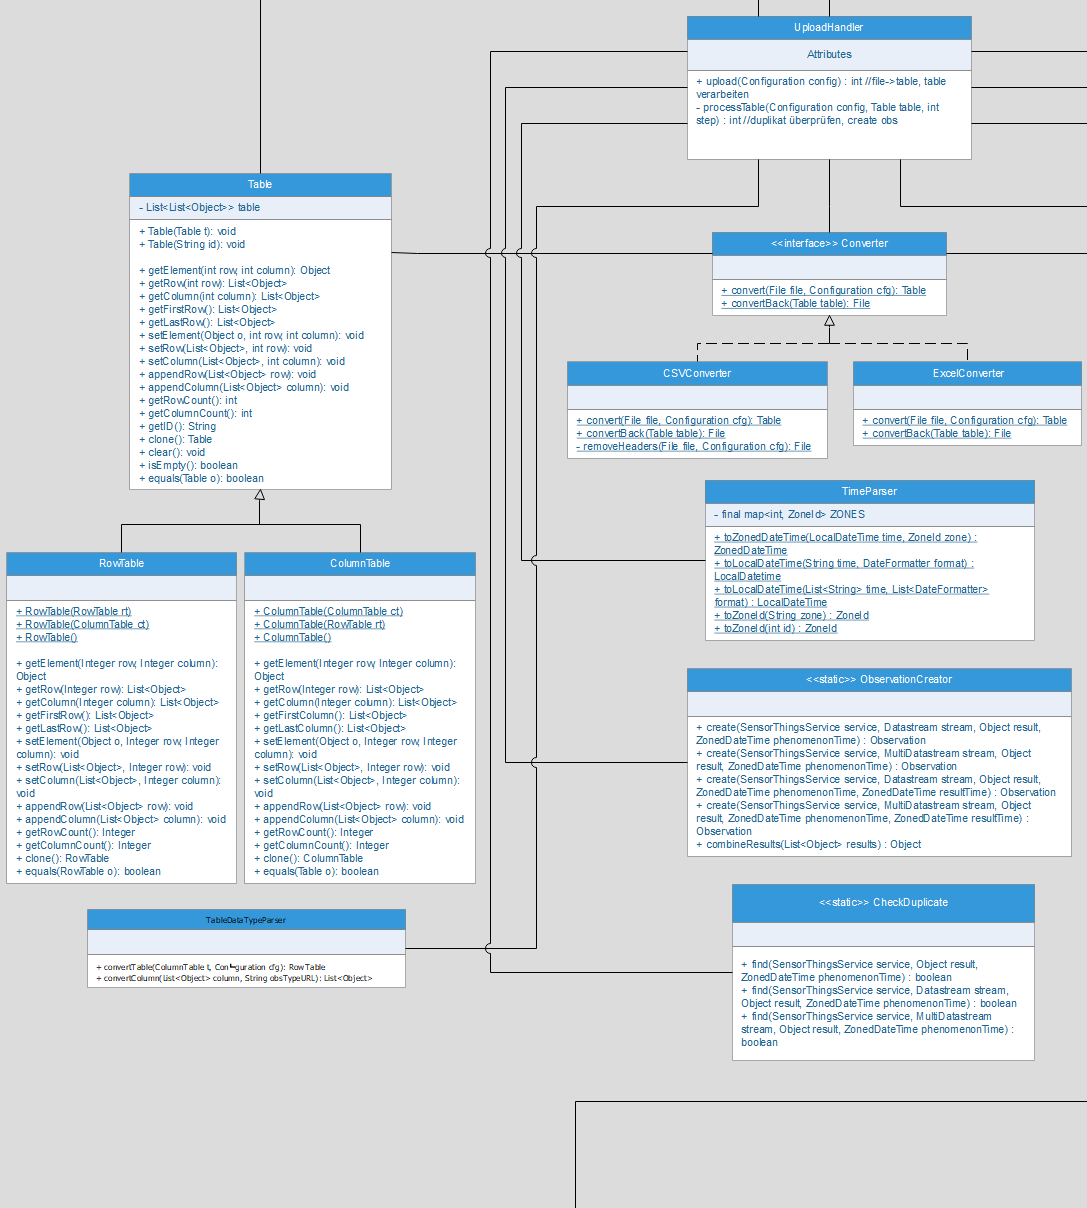
\includegraphics[scale=0.6]{uml/screenshots/upload}
\caption{Klassen für den Datenimport}
\end{figure}
\clearpage
\subsection{UploadHandler}
Die Klasse UploadHandler ist für die Überwachung des Ablaufs eines Imports von Daten aus einem File auf den FROST-Server zuständig.

\paragraph{Attribute}
\paragraph{Methoden}
\begin{itemize}
\item \textit{public String upload(Configuration config)} Verwaltet den Upload von Daten auf den FROST-Server mithilfe der Konfiguration (lädt die Quelldatei, bringt die Daten in die interne Darstellung und verarbeitet diese dann)
\item \textit{public String processTable(Configuration config, Table table, int step)} Liest aus der übergebenen Table die mithilfe der Konfiguration zeilenweise die Daten aus und erstellt damit Observations, überprüft diese auf Duplikate und erstellt sie auf dem FROST-Server
\end{itemize}

\clearpage
\input{content/klassen/Table/Interface-Table}
\clearpage
\subsection{RowTable implements Table}	
Repräsentiert eine 2-dimensionale Tabelle bestehend aus Zeilen und Spalten mit dem Fokus auf zeilenweise Verarbeitung. Der Inhalt der Tabellenelemente ist nicht beschränkt.
	
	
\paragraph{Attribute}

\begin{itemize}
	\item[-] \textit{List{<List<Object>}> rowTable} \\
	Speichert die Daten der Tabelle, jedes Listenelement enthält eine weitere Liste, welche die Elemente der Tabelle hält. \\
	Die "äußere" Listenelemente repräsentieren die Zeilen der Tabelle, die inneren Listenelemente die Spalten.
\end{itemize}


\paragraph{Konstruktoren}

\begin{enumerate}[+]
	\item \textit{RowTable(RowTable rt)} \\
	Erstellt eine RowTable-Instanz aus einer anderen RowTable-Instanz \\
	Dabei werden alle inneren Listen auf die selbe Länge verlängert und mit NULL aufgefüllt, damit die Tabelle immer gleich viele Spalten besitzt	
	\begin{enumerate}[$\bullet$]
		\item \textit{RowTable rt}: Die RowTable-Instanz aus der ein neuer RowTable erstellt wird, kann NULL sein
	\end{enumerate}
	\vspace{-0.2cm}
	
	
	\item \textit{RowTable(ColumnTable ct)} \\
	Erstellt eine RowTable-Instanz aus einer ColumnTable-Instanz \\
	Dabei werden alle inneren Listen auf die selbe Länge verlängert und mit NULL aufgefüllt, damit die Tabelle immer gleich viele Spalten besitzt	
	\begin{enumerate}[$\bullet$]
		\item \textit{ColumnTable ct}: Die ColumnTable-Instanz aus der ein neuer RowTable erstellt wird, kann NULL sein
	\end{enumerate}
	\vspace{-0.2cm}
	
	\item \textit{RowTable()} \\
	Erstellt einen neuen RowTable mit leerer Tabelle
\end{enumerate}


\paragraph{Methoden}

\begin{enumerate}[+]
	\item \textit{getElement(int row, int column): Object} \\
	Gibt ein einzelnes Element der Tabelle an der angegebenen Stelle zurück
	\begin{enumerate}[$\bullet$]
		\item \textit{int row}: Die Zeile an der das Element liegt, darf nicht NULL sein
		\item \textit{int column}: Die Spalte an der das Element liegt, darf nicht NULL sein
	\end{enumerate}
	\vspace{-0.2cm}
	\begin{enumerate}[$\circ$]
		\item \textit{Object}: Das Element an der Stelle
	\end{enumerate}
	
	\item \textit{getRow(int row): List<Object>} \\
	Gibt eine ganze Zeile zurück
	\begin{enumerate}[$\bullet$]
		\item \textit{int row}: Die Position der Zeile, darf nicht NULL sein
	\end{enumerate}
	\vspace{-0.2cm}
	\begin{enumerate}[$\circ$]
		\item \textit{List<Object>}: die Zeile als Liste
	\end{enumerate}
	
	\item \textit{getColumn(int column): List<Object>} \\
	Gibt eine ganze Spalte zurück
	
	\begin{enumerate}[$\bullet$]
		\item \textit{int column}: Die Position der Spalte, darf nicht NULL sein
	\end{enumerate}
	\vspace{-0.2cm}
	\begin{enumerate}[$\circ$]
		\item \textit{List<Object>}: die Spalte als Liste
	\end{enumerate}
	
	\item \textit{getFirstRow(): List<Object>} \\
	Gibt die erste Zeile zurück
	\vspace{-0.2cm}
	\begin{enumerate}[$\circ$]
		\item \textit{List<Object>}: Die erste Zeile
	\end{enumerate}
	
	\item \textit{getLastRow(): List<Object>} \\
	Gibt die letzte Zeile zurück
	\vspace{-0.2cm}
	\begin{enumerate}[$\circ$]
		\item \textit{List<Object>}: Die letzte Zeile
	\end{enumerate}
	
	\item \textit{setElement(Object o, int row, int column): void} \\
	Ersetzt ein Element der Tabelle mit einem neuen Element
	\begin{enumerate}[$\bullet$]
		\item \textit{Object o}: Das neue Element, darf NULL sein
		\item \textit{int row}: Die Zeile des Elements
		\item \textit{int column}: Die Spalte des Elements
	\end{enumerate}
	\vspace{-0.2cm}
	
	\item \textit{setRow(List<Object> row, int pos): void} \\
	Ersetzt eine Zeile mit einer neuen Zeile
	\begin{enumerate}[$\bullet$]
		\item \textit{List<Object> row}: Die neue Zeile als Liste, darf NULL sein
		\item \textit{int pos}: Die Position der zu ersetzenden Zeile
	\end{enumerate}
	\vspace{-0.2cm}
	
	\item \textit{setColumn(List<Object> column, int pos): void} \\
	Ersetzt eine Spalte mit einer neuen Spalte
	\begin{enumerate}[$\bullet$]
		\item \textit{List<Object> column}: Die neue Spalte als Liste, darf NULL sein
		\item \textit{int pos}: Die Position der zu ersetzen Spalte
	\end{enumerate}
	\vspace{-0.2cm}
	
	\item \textit{remove(int row, int column): void} \\
	Ersetzt ein Element mit NULL
	\begin{enumerate}[$\bullet$]
		\item \textit{int row}: Die Zeile des Elements
		\item \textit{int column}: Die Spalte des Elements
	\end{enumerate}
	\vspace{-0.2cm}
	
	\item \textit{appendRow(List<Object> row): void} \\
	Fügt eine neue Zeile hinter der letzten bestehenden Zeile ein
	\begin{enumerate}[$\bullet$]
		\item \textit{List<Object> row}: Die einzufügende Zeile als Liste
	\end{enumerate}
	\vspace{-0.2cm}
	
	\item \textit{appendColumn(List<Object> column): void} \\
	Fügt eine neue Spalte hinter der letzten bestehenden Spalte ein
	\begin{enumerate}[$\bullet$]
		\item \textit{List<Object> column}: Die einzufügende Spalte als Liste
	\end{enumerate}
	\vspace{-0.2cm}
	
	\item \textit{getRowCount(): int} \\
	Gibt die Anzahl Zeilen zurück
	\vspace{-0.2cm}
	\begin{enumerate}[$\circ$]
		\item \textit{int}: Die Anzahl Zeilen
	\end{enumerate}
	
	\item \textit{getColumnCount(): int} \\
	Gibt die Anzahl Spalten zurück
	\vspace{-0.2cm}
	\begin{enumerate}[$\circ$]
		\item \textit{int}: Die Anzahl Spalten
	\end{enumerate}
	
	\item \textit{clone(): Table} \\
	Erstellt eine ganze Kopie der Tabelle
	\vspace{-0.2cm}
	\begin{enumerate}[$\circ$]
		\item \textit{Table}: die Kopie der Tabelle als neue Table-Instanz
	\end{enumerate}
	
	\item \textit{clear(): void} \\
	Löscht die Tabelle komplett und ersetzt sie gegen NULL
	
	\item \textit{isEmpty(): boolean} \\
	Gibt zurück ob die Tabelle leer ist
	\vspace{-0.2cm}
	\begin{enumerate}[$\circ$]
		\item \textit{boolean}: true wenn die Tabelle leer oder NULL ist
	\end{enumerate}
	
	\item \textit{compare(Table o): boolean} \\
	Vergleicht die Table-Instanz mit einer anderen Instanz
	\begin{enumerate}[$\bullet$]
		\item \textit{Table o}: Die andere zu vergleichede Table-Instanz
	\end{enumerate}
	\vspace{-0.2cm}
	\begin{enumerate}[$\circ$]
		\item \textit{boolean}: true, wenn alle Einträge gleich sind, sonst false
	\end{enumerate}
\end{enumerate}
\clearpage
\subsection*{ColumnTable extends \hyperref[Table]{Table}}\label{colTable}

Repräsentiert eine 2-dimensionale Tabelle bestehend aus Zeilen und Spalten mit dem Fokus auf spaltenweise Verarbeitung. Der Inhalt der Tabellenelemente ist nicht beschränkt.


\paragraph{Attribute geerbt von \hyperref[Table]{Table}}

\begin{itemize}
	\item[-] \textit{table: List{<List<Object>}>} \\
	Speichert die Daten der Tabelle, jedes Listenelement enthält eine weitere Liste, welche die Elemente der Tabelle hält. \\
	Die äußeren Listenelemente repräsentieren die Spalten der Tabelle, die inneren Listenelemente die Zeilen.
\end{itemize}


\paragraph{Konstruktoren}

\begin{enumerate}[+]
	\item \textit{ColumnTable(ColumnTable ct)} \\
	Erstellt eine Table-Instanz aus einer ColumnTable \\
	Dabei werden alle äußeren Listen auf die selbe Länge verlängert und mit NULL aufgefüllt, damit die Tabelle immer gleich viele Spalten besitzt	
	\begin{enumerate}[$\bullet$]
		\item \textit{Table t}: Die Table-Instanz aus der ein neuer Table erstellt wird, kann NULL sein
	\end{enumerate}
	\vspace{-0.2cm}
	
	\item \textit{ColumnTable(RowTable rt)} \\
	Erstellt eine ColumnTable-Instanz aus einer RowTable \\
	Dabei werden alle äußeren Listen auf die selbe Länge verlängert und mit NULL aufgefüllt, damit die Tabelle immer gleich viele Spalten besitzt	
	\begin{enumerate}[$\bullet$]
		\item \textit{Table t}: Die Table-Instanz aus der ein neuer Table erstellt wird, kann NULL sein
	\end{enumerate}
	\vspace{-0.2cm}
	
	\item \textit{ColumnTable()} \\
	Erstellt einen neuen ColumnTable mit leerer Tabelle
\end{enumerate}

		
\paragraph{Methoden}

\begin{enumerate}[+]
	\item \textit{getElement(int row, int column): Object} \\
	Gibt ein einzelnes Element der Tabelle an der angegebenen Stelle zurück
	\begin{enumerate}[$\bullet$]
		\item \textit{int row}: Die Zeile an der das Element liegt, darf nicht NULL sein
		\item \textit{int column}: Die Spalte an der das Element liegt, darf nicht NULL sein
	\end{enumerate}
	\vspace{-0.2cm}
	\begin{enumerate}[$\circ$]
		\item \textit{Object}: Das Element an der Stelle
	\end{enumerate}
	
	\item \textit{getRow(int row): List<Object>} \\
	Gibt eine ganze Zeile zurück
	\begin{enumerate}[$\bullet$]
		\item \textit{int row}: Die Position der Zeile, darf nicht NULL sein
	\end{enumerate}
	\vspace{-0.2cm}
	\begin{enumerate}[$\circ$]
		\item \textit{List<Object>}: die Zeile als Liste
	\end{enumerate}
	
	\item \textit{getColumn(int column): List<Object>} \\
	Gibt eine ganze Spalte zurück
	\begin{enumerate}[$\bullet$]
		\item \textit{int column}: Die Position der Spalte, darf nicht NULL sein
	\end{enumerate}
	\vspace{-0.2cm}
	\begin{enumerate}[$\circ$]
		\item \textit{List<Object>}: die Spalte als Liste
	\end{enumerate}
	
	\item \textit{getFirstColumn(): List<Object>} \\
	Gibt die erste Spalte zurück
	\vspace{-0.2cm}
	\begin{enumerate}[$\circ$]
		\item \textit{List<Object>}: Die erste Spalte
	\end{enumerate}
	
	\item \textit{getLastColumn(): List<Object>} \\
	Gibt die letzte Spalte zurück
	\vspace{-0.2cm}
	\begin{enumerate}[$\circ$]
		\item \textit{List<Object>}: Die letzte Spalte
	\end{enumerate}
	
	\item \textit{setRow(List<Object> row, int pos): void} \\
	Ersetzt eine Zeile mit einer neuen Zeile
	\begin{enumerate}[$\bullet$]
		\item \textit{List<Object> row}: Die neue Zeile als Liste, darf NULL sein
		\item \textit{int pos}: Die Position der zu ersetzenden Zeile
	\end{enumerate}
	\vspace{-0.2cm}
	
	\item \textit{setColumn(List<Object> column, int pos): void} \\
	Ersetzt eine Spalte mit einer neuen Spalte
	\begin{enumerate}[$\bullet$]
		\item \textit{List<Object> column}: Die neue Spalte als Liste, darf NULL sein
		\item \textit{int pos}: Die Position der zu ersetzen Spalte
	\end{enumerate}
	\vspace{-0.2cm}
	
	\item \textit{appendRow(List<Object> row): void} \\
	Fügt eine neue Zeile hinter der letzten bestehenden Zeile ein
	\begin{enumerate}[$\bullet$]
		\item \textit{List<Object> row}: Die einzufügende Zeile als Liste
	\end{enumerate}
	\vspace{-0.2cm}
	
	\item \textit{appendColumn(List<Object> column): void} \\
	Fügt eine neue Spalte hinter der letzten bestehenden Spalte ein
	\begin{enumerate}[$\bullet$]
		\item \textit{List<Object> column}: Die einzufügende Spalte als Liste
	\end{enumerate}
	\vspace{-0.2cm}
	
	\item \textit{getRowCount(): int} \\
	Gibt die Anzahl Zeilen zurück
	\vspace{-0.2cm}
	\begin{enumerate}[$\circ$]
		\item \textit{int}: Die Anzahl Zeilen
	\end{enumerate}
	
	\item \textit{getColumnCount(): int} \\
	Gibt die Anzahl Spalten zurück
	\vspace{-0.2cm}
	\begin{enumerate}[$\circ$]
		\item \textit{int}: Die Anzahl Spalten
	\end{enumerate}
	
	\item \textit{clone(): ColumnTable} \\
	Erstellt eine ganze Kopie der Tabelle
	\vspace{-0.2cm}
	\begin{enumerate}[$\circ$]
		\item \textit{Table}: die Kopie der Tabelle als neue ColumnTable-Instanz
	\end{enumerate}
	
	\item \textit{compare(Table o): boolean} \\
	Vergleicht die ColumnTable-Instanz mit einer anderen Instanz
	\begin{enumerate}[$\bullet$]
		\item \textit{Table o}: Die andere zu vergleichede Table-Instanz
	\end{enumerate}
	\vspace{-0.2cm}
	\begin{enumerate}[$\circ$]
		\item \textit{boolean}: true, wenn alle Einträge gleich sind, sonst false
	\end{enumerate}
\end{enumerate}

\clearpage
\subsection{<{<{interface}>}> Converter}
Stellt Methoden zur konvertierung einer Datei aus dem File-Format in das RowTable-Format für die interne Repräsentation und wieder zurück bereit. \\

\paragraph{Methoden}
\begin{enumerate}[+]
	\item \underline{\textit{convert(File file, configuration cfg): RowTable}} \\
	Konvertiert eine Tabellen-Datei in eine Instanz der Klasse RowTable
	
	\begin{enumerate}[$\bullet$]
		\item \textit{File file}: Die zu konvertierende Datei, kann NULL sein, muss sonst aber eine Tabelle repräsentieren
		\item \textit{Configuration cfg}: Die zu nutzende Konfiguration
	\end{enumerate}
	\vspace{-0.2cm}
	\begin{enumerate}[$\circ$]
		\item \textit{RowTable}: die RowTable-Instanz die die Tabelle repräsentiert
	\end{enumerate}

	\item \underline{\textit{convertBack(RowTable table, Configuration cfg): File}} \\
	Konvertiert eine RowTable-Instanz wieder zurück in eine Datei, die gespeichert werden kann
	\begin{enumerate}[$\bullet$]
		\item \textit{RowTable table}: Die zu konvertierende RowTable-Instanz
		\item \textit{Configuration cfg}: Die zu nutzende Konfiguration
	\end{enumerate}
	\vspace{-0.2cm}
	\begin{enumerate}[$\circ$]
		\item \textit{File}: Die Datei
	\end{enumerate}
\end{enumerate}
\clearpage
\subsection{CSVConverter implements Converter}
Konvertiert eine Datei aus dem File-Format in das RowTable-Format für die interne Repräsentation und wieder zurück \\
Konvertiert nur CSV-Dateien. \\

\paragraph{Methoden}

\begin{enumerate}[+]
	\item \underline{\textit{convert(File file, Configuration cfg): RowTable}} \\
	Konvertiert eine Tabellen-Datei im CSV-Format in eine Instanz der Klasse Table
	
	\begin{enumerate}[$\bullet$]
		\item \textit{File file}: Die zu konvertierende Datei, kann NULL sein, muss ansonsten aber eine Tabelle im CSV-Format repräsentieren
		\item \textit{Configuration cfg}: Die zu nutzende Konfiguration, diese stellt u.a. die zu entfernenden Kopfzeilen, die Magic Numbers und das Trennsymbol bereit
	\end{enumerate}
	\vspace{-0.2cm}
	\begin{enumerate}[$\circ$]
		\item \textit{RowTable}: die RowTable-Instanz die die Tabelle repräsentiert
	\end{enumerate}
	
	\item \underline{\textit{convertBack(RowTable table, Configuration cfg): File}} \\
	Konvertiert eine Table-Instanz wieder zurück in eine Datei, die gespeichert werden kann
	\begin{enumerate}[$\bullet$]
		\item \textit{RowTable table}: Die zu konvertierende RowTable-Instanz
		\item \textit{Configuration cfg}: Die zu nutzende Konfiguration, die u.a. das Trennsymbol und die Kopfzeilen, die wieder hinzugefügt werden, bereitstellt
	\end{enumerate}
	\vspace{-0.2cm}
	\begin{enumerate}[$\circ$]
		\item \textit{File}: Die CSV-Datei
	\end{enumerate}

	\item \underline{\textit{removeHeaders(File file, Configuration cfg): File}} \\
	Entfernt die Kopfzeilen der CSV-Datei, welche durch die Konfiguration festgelegt sind
	\begin{enumerate}[$\bullet$]
		\item \textit{File file}: Die CSV-Datei von der die Kopfzeilen entfernt werden sollen
		\item \textit{Configuration cfg}: Die Konfiguration, die die Anzahl Kopfzeilen enthält
	\end{enumerate}
	\vspace{-0.2cm}
	\begin{enumerate}[$\circ$]
		\item \textit{File}: Die selbe CSV-Datei, nur ohne Kopfzeilen
	\end{enumerate}
\end{enumerate}

\clearpage
\subsection{ExcelConverter implements Converter}
Konvertiert eine Datei aus dem File-Format in das RowTable-Format für die interne Repräsentation und wieder zurück \\

Konvertiert nur Excel-Dateien. \\

\paragraph{Methoden}
\begin{enumerate}[+]
	\item \underline{\textit{convert(File file): RowTable}} \\
	Konvertiert eine Tabellen-Datei im Excel-Format in eine Instanz der Klasse RowTable.
	Jeder Wert der Excel-Tabelle behält seinen Datentyp bzw wird in den entsprechenden Java-Datentyp umgewandelt.
	
	\begin{enumerate}[$\bullet$]
		\item \textit{File file}: Die zu konvertierende Datei, kann NULL sein, muss ansonsten aber eine Tabelle im Excel-Format repräsentieren
		\item \textit{Configuration cfg}: Die zu nutzende Konfiguration
	\end{enumerate}
	\vspace{-0.2cm}
	\begin{enumerate}[$\circ$]
		\item \textit{RowTable}: die RowTable-Instanz die die Tabelle repräsentiert
	\end{enumerate}
	
	\item \underline{\textit{convertBack(RowTable table, Configuration cfg): File}} \\
	Konvertiert eine RowTable-Instanz wieder zurück in eine Excel-Datei, die gespeichert werden kann.
	Die Datentypen werden -wenn möglich- aus dem Java-Datentyp wieder in den Excel-Datentyp zurück-konvertiert.
	Siehe auch: \href{https://support.office.com/en-us/article/data-types-in-data-models-e2388f62-6122-4e2b-bcad-053e3da9ba90#__toc327893213}{Datentypen in MS Excel}
	\begin{enumerate}[$\bullet$]
		\item \textit{RowTable table}: Die zu konvertierende RowTable-Instanz
		\item \textit{Configuration cfg}: Die zu nutzende Konfiguration
	\end{enumerate}
	\vspace{-0.2cm}
	\begin{enumerate}[$\circ$]
		\item \textit{File}: Die Excel-Datei
	\end{enumerate}
\end{enumerate}


\clearpage

\subsection{CreateObservations}

\paragraph{Beschreibung}
Hier werden die Observations erstellt, die anschließend auf den Frost-Server hochgeladen werden können.
Dazu werden die Daten aus der internen Tabellendarstellung gelesen und daraus zeilenweise Observations erstellt, mit der Duplikatklasse auf Duplikate überprüft und anschließend hochgeladen

\paragraph{Attribute}
- Konfigurationsklasse

\paragraph{Methoden}

\begin{itemize}
\item + processTable(Table table, int step) : void
nimmt die Table entgegen und schreibt die Daten in Observations, step sagt wie viele zeilen auf einmal abgearbeitet werden, bevor observations hochgeladen werden
\item - createObs(String name, Object result, ZonedDateTime time) : Observation
\item - createObs(String name, Object result, List<String> time, List<Formatter> format, String zone) : Observation
methoden zum Erstellen von Observations mit verschiedenen Parametern
\item - combineResults(List<Object> results) : Object
erstellt aus mehreren results ein einziges result-Object
\end{itemize}
\clearpage
\subsection{CheckDuplicate}

Diese Klasse enthält die Funktionalität zur Überprüfung einer Observation auf Duplikate auf dem FROST-Server.
Zwei Observations sind Duplikate, falls das Ergebnis und die Beobachtungszeit übereinstimmen.

\paragraph{Methoden}
	
	\begin{enumerate}[+]
\item \underline{\textit{find(ZonedDateTime time, Object result) : boolean}}\\
Sucht eine Observation auf dem FROST-Server mit gegebener Beobachtungszeit und Result und gibt true im Erfolgsfall zurück, sonst false
\begin{enumerate}[$\bullet$]
\item \textit{ZonedDateTime time:} die Beobachtungszeit der Observation
\item \textit{Object result:} der Wert der Observation
\end{enumerate}
\vspace{-0.2cm}
\begin{enumerate}[$\circ$]
\item \textit{boolean:} Angabe, ob Observation gefunden wurde
\end{enumerate}
	
\item \underline{\textit{find(Datastream stream, ZonedDateTime time, Object result) : boolean}}\\
Sucht eine Observation zu dem Datastream auf dem FROST-Server mit gegebener Beobachtungszeit und Result und gibt true im Erfolgsfall zurück, sonst false

\begin{enumerate}[$\bullet$]
\item \textit{Datastream stream:} der Datastream, zu der Observation
\item \textit{ZonedDateTimetime:} die Beobachtungszeit der Observation
\item \textit{Object result:} der Wert der Observation
\end{enumerate}
\vspace{-0.2cm}
\begin{enumerate}[$\circ$]
\item \textit{boolean:} Angabe, ob Observation gefunden wurde
\end{enumerate}

\item \underline{\textit{find(MultiDatastream stream, ZonedDateTime time, Object result) : boolean}}\\
Sucht eine Observation zu dem MultiDatastream auf dem FROST-Server mit gegebener Beobachtungszeit und Result und gibt true im Erfolgsfall zurück, sonst false

\begin{enumerate}[$\bullet$]
\item \textit{MultiDatastream stream:} der MultiDatastream, zu der Observation
\item \textit{ZonedDateTimetime:} die Beobachtungszeit der Observation
\item \textit{Object result:} der Wert der Observation
\end{enumerate}
\vspace{-0.2cm}
\begin{enumerate}[$\circ$]
\item \textit{boolean:} Angabe, ob Observation gefunden wurde
\end{enumerate}

\end{enumerate}
\clearpage
\subsection*{TimeParser}\label{timeParser}

Diese Klasse stellt die Funktionalität zur Konvertierung von Zeitformaten in das vom FROST-Server verwendete ZonedDateTime-Format bereit. \\
Je nach (teilweise) schon bestehenden Zeitformaten sollen dafür verschiedene Methoden zur Verfügung stehen.


\paragraph{Methoden}
\begin{enumerate}[+]
	
	\item \underline{\textit{toZonedDateTime(LocalDateTime time, ZoneId zone) : ZonedDateTime}}\\
	Erstellt eine ZonedDateTime aus einer LocalDateTime und Zeitzone
	\begin{enumerate}[$\bullet$]
		\item \textit{LocalDateTime time}: die LocalDateTime für die ZonedDateTime
		\item \textit{ZoneId zone:} die Zeitzone für die ZonedDateTime
	\end{enumerate}
	\vspace{-0.2cm}
	\begin{enumerate}[$\circ$]
		\item \textit{ZonedDateTime:} die erstellte ZonedDateTime
	\end{enumerate}
	
	\item \underline{\textit{toLDT(String time, DateTimeFormatter format) : LocalDateTime}}\\
	Konvertiert einen String über das gegebene Format in die zugehörige LocalDateTime
	\begin{enumerate}[$\bullet$]
		\item \textit{String time}: der String, aus dem die Zeit erstellt wird
		\item \textit{DateTimeFormatter format}: das Format für den String
	\end{enumerate}
	\vspace{-0.2cm}
	\begin{enumerate}[$\circ$]
		\item \textit{LocalDateTime:} die erstellte LocalDateTime
	\end{enumerate}
	
	\item \underline{\textit{toLDT(List<String> time, List<DateTimeFormatter> format) : LocalDateTime}}\\
	Konvertiert mehrere Strings über die Formate in die zugehörige LocalDatetime
	\begin{enumerate}[$\bullet$]
		\item \textit{List<String> time:} die Strings, aus denen die Zeit erstellt wird
		\item \textit{List<DateTimeFormatter> format:} die Formate für die Strings
	\end{enumerate}
	\vspace{-0.2cm}
	\begin{enumerate}[$\circ$]
		\item \textit{LocalDateTime:} die erstellte LocalDateTime
	\end{enumerate}
	
	\item \underline{\textit{toZoneId(String zone) : ZoneId}}\\
	Konvertiert einen String in die zugehörige Zeitzone
	\begin{enumerate}[$\bullet$]
		\item \textit{String zone:} Zone als String
	\end{enumerate}
	\vspace{-0.2cm}
	\begin{enumerate}[$\circ$]
		\item \textit{ZoneId:} die erstellte ZoneId
	\end{enumerate}

\end{enumerate}
\clearpage
\subsection{TableDataTypeParser}

Diese Klasse konvertiert die Datentypen einer ColumnTable-Tabelle in die Datentypen die nach der Konfiguration für den (Multi)Datastream benötigt werden.

\paragraph{Attribute}

\paragraph{Methoden}

\begin{enumerate}[+]
	\item \underline{\textit{convertTable(ColumnTable t, Configuration cfg): RowTable}} \\	
	\begin{enumerate}[$\bullet$]
		\item \textit{ColumnTable t}: Die RowTable-Instanz aus der ein neuer RowTable erstellt wird, kann NULL sein
		\item \textit{Configuration cfg}: Die zu Nutzende Konfiguration, die die benötigten Datentypen an den richtigen Spalten bereitstellt
	\end{enumerate}
	\vspace{-0.2cm}
	\begin{enumerate}[$\circ$]
		\item \textit{RowTable}: Die konvertierte Tabelle
	\end{enumerate}

	\item \underline{\textit{convertColumn(List<Object> column, String obsTypeURL): List<Object>}} \\
	Konvertiert eine Spalte der Tabelle in den durch den ObservationType angegebenen Datentyp
	\begin{enumerate}[$\bullet$]
		\item \textit{List<Object> column}: Die zu konvertierende Spalte als Liste von Objekten
		\item \textit{String obsTyeURL}: Die URL des ObservationTypes, die den Datentyp festegt
	\end{enumerate}
	\vspace{-0.2cm}
	\begin{enumerate}[$\circ$]
		\item \textit{List<Object>}: Die konvertierte Spalte
	\end{enumerate}
\end{enumerate}


\clearpage
\subsection{Konfigurationen}
\begin{figure}[!h]
\centering
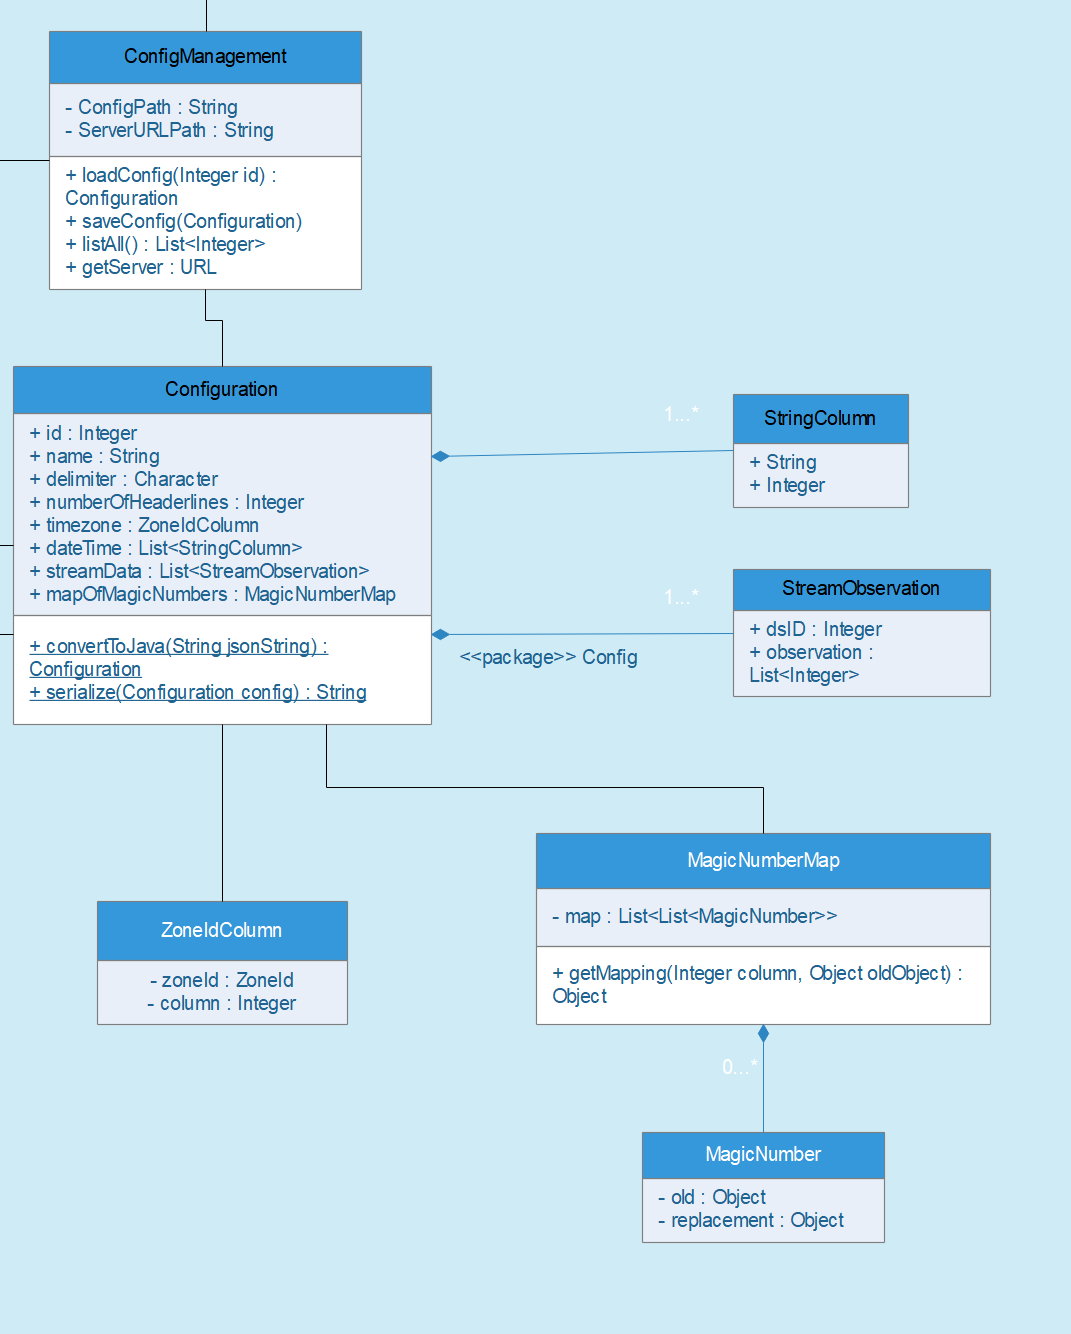
\includegraphics[scale=0.6]{uml/screenshots/configuration}
\caption{Klassen für das Konfigurations-Management}
\end{figure}
\clearpage

\subsection{StringColumn}
Diese Klasse stellt ein Tupel aus einem String und einer Spaltennummer dar.
Diese Klasse wird dazu verwendet eine DateTime anzugeben. \\Diese hat einen Regex-String und eine Spaltennummer, in welcher der zu importierende Wert zu finden ist.
\paragraph{Attribute}
\begin{enumerate}[-]
	\item \textit{string : String} Ein String
	\item \textit{column : Integer} Eine Spaltennummer
\end{enumerate} 

\paragraph{Konstruktoren}
\begin{enumerate}[+]
	\item \textit{StringColumn(String s, Integer column)} \\
	
	\begin{enumerate}[$\bullet$]
		\item \textit{String s}: 
		\item \textit{Integer column}:
	\end{enumerate}
\end{enumerate}







\subsection{StreamObservation}
Diese Klasse speichert einen Datastream zusammen mit einer Liste aus Spaltenangaben, welche anzeigen, wo die Observations auszulesen sind.
\paragraph{Attribute} 
\begin{enumerate}[-]
	\item \textit{dsID: Integer} ID eines (Multi-) Datastreams
	\item \textit{observation: List<Integer>} Spaltenangaben
\end{enumerate}

\paragraph{Konstruktoren}
\begin{enumerate}[+]
	\item \textit{StreamObservation(Integer dsID, List<Integer> observation)} \\
	
	\begin{enumerate}[$\bullet$]
		\item \textit{Integer dsID}:
		\item \textit{List<Integer> observation}:
	\end{enumerate}
\end{enumerate}






\subsection{ZoneIdColumn}
Diese Klasse stellt ein Tupel aus einer ZoneId und einer Spaltennummer dar.\\
Sie wird verwendet um die variableTimeZone mit der staticTimeZone zu verbinden, so wird diese Klasse zum Beispiel als Rückgabeparameter bei getTimezone verwendet.

\paragraph{Attribute}
\begin{enumerate}[-]
	\item \textit{zoneId : ZoneId} Die ID einer Zeitzone
	\item \textit{column : Integer} Spaltennummer
\end{enumerate}

\paragraph{Konstruktoren}
\begin{enumerate}[+]
	\item \textit{ZoneIdColumn(ZoneId zoneId, Integer column)} \\
	
	\begin{enumerate}[$\bullet$]
		\item \textit{ZoneId zoneId:} 
		\item \textit{Integer column:} 
	\end{enumerate}
\end{enumerate}












\subsection{Configuration}
Diese Klasse stellt eine Nutzer-erstellte Konfiguration dar. 
Sie speichert alle notwendigen Daten und stellt "{Getter}"{-Methoden} für einen vereinfachten Zugriff auf Daten bereit.

\paragraph{Attribute}

\begin{enumerate}[-]
	\item \textit{id : Integer}: Hier wird die ID der Konfiguration gespeichert. Die ID wird automatisch generiert
	
	\item \textit{name : String}: Hier wird der Name der Konfiguration gespeichert
	
	\item \textit{delimiter : Character}: Falls eine CSV-Datei importiert werden soll, muss ein Trennsymbol für die Spalten gewählt werden
	
	\item \textit{numberOfHeaderlines : Integer}: In einem CSV-Dokument gibt es Kopfzeilen, welche für den Import irrelevant sind. Die Anzahl dieser Zeilen wird hier gespeichert
	
	\item \textit{timezone : ZoneIdColumn}: Hier wird die Zeitzone gespeichert
	
	\item \textit{dateTime : List<StringColumn>}: Hier wird eine Liste aus Datumsformaten mit einer zugehörigen Spalte gespeichert 
	
	\item \textit{streamData : List<StreamObseration>}: In dieser Liste werden die Datastreams zusammen mit den Spalten gespeichert, aus welchen die Daten extrahiert werden
	
	\item \textit{mapOfMagicNumbers : MagicNumberMap}: Hier wird das Mapping für Sonderzeichen gespeichert. Sonderzeichen sollen nicht auf dem FROST-Server gespeichert werden und haben eine spezielle Bedeutung
\end{enumerate}

\paragraph{Konstruktoren}
\begin{enumerate}[+]
	\item \textit{Configuration(Integer id, String name, Character delimiter, Integer numberOfHeaderlines, ZoneIdColumn timezone, List<StringColumn> dateTime, List<StreamObservation> streamData, MagicNumberMap mapOfMagicNumbers)} Dieser Konstruktor erstellt aus den gegebenen Parametern eine vollständig ausgefüllte Configuration
	\begin{enumerate}[$\bullet$]
		\item \textit{Integer id}: ID der Konfiguration
		\item \textit{String name}: Name der Konfiguration
		\item \textit{Character delimiter}: Spaltentrennsymbol
		\item \textit{Integer numberOfHeaderlines}: Anzahl der Kopfzeilen
		\item \textit{ZoneIdColumn timezone}: Zeitzone oder Splatennummer der Zone
		\item \textit{List<StringColumn> dateTime}: Liste für Zeitangaben
		\item \textit{List<StreamObservation> streamData}: Liste aus Streams mit dazugehörigen Spaltennummern für Observations
		\item \textit{MagicNumberMap mapOfMagicNumbers}: Mapping für Sonderzeichen
	\end{enumerate}
\end{enumerate}

\paragraph{Methoden}
\begin{enumerate}[+]
	\item \textit{\underline{convertToJava(String jsonString): Configuration}} Diese Methode generiert aus einem JSON-String eine Configuration
	\begin{enumerate}[$\bullet$]
		\item \textit{String jsonString:} Der String, in dem das JSON-Objekt kodiert ist
	\end{enumerate}
	\begin{enumerate}[$\circ$]
		\item \textit{Configuration}: Die generierte Konfiguration
	\end{enumerate}
	
	\item \textit{\underline{serialize(Configuration config): String}} Diese Methode generiert aus einer Konfiguration ein JSON-String
	\begin{enumerate}[$\bullet$]
		\item \textit{Configuration config}: Die Konfiguration, welche in einen String überführt werden soll
	\end{enumerate}
	\begin{enumerate}[$\circ$]
		\item \textit{String:} Das generierte JSON-Objekt als String
	\end{enumerate}
\end{enumerate}

\clearpage
\subsection*{MagicNumber}\label{magic}
Klasse zum Abspeichern einer Zuordnung für die Ersetzung von \string"Magic Numbers\string".

\paragraph{Attribute}
\begin{enumerate}[-]
	\item \textit{old: Object} In der Quelldatei vorkommender Wert
	\item \textit{replacement: Object} Neuer Wert, der den alten ersetzt
\end{enumerate}


\subsection*{MagicNumberMap}\label{magicMap}
Klasse zum Abspeichern mehrerer MagicNumbers bezüglich einer Spalte

\paragraph{Attribute}
\begin{enumerate}[-]
	\item \textit{map: List<List<MagicNumber>{}>} Die äußere Liste stellt die Spalten dar. In der inneren Liste werden die verschiedenen Mappings für die Spalte gespeichert
\end{enumerate}

\paragraph{Methoden}
\begin{enumerate}[+]
	\item \textit{getMapping(int column, Object oldObject) : Object} Gibt das Objekt aus, auf das oldObject und column gemappt werden
	
	\begin{enumerate}[$\bullet$]
		\item \textit{int column} Die Spalte aus der oldObject stammt
		\item \textit{Object oldObject:} Ein Object welches abgebildet werden soll
	\end{enumerate}
	\vspace{-0.2cm}
	\begin{enumerate}[$\circ$]
		\item \textit{Object:} Das Objekt auf welches oldObject abgebildet wird
	\end{enumerate}
\end{enumerate}
\clearpage

\subsection{ConfigManager}
Diese Klasse ist für die Verwaltung der Konfigurationen zuständig.
\paragraph{Attribute}
\begin{enumerate}[-]
	\item \textit{configPath : String} Speichert den Weg zu dem Ordner, in dem die Konfigurationen gespeichert sind
	
	\item \textit{serverURLPath : String} Hier wird gespeichert, wo die Datei mit der Zielserver-URL liegt.		
\end{enumerate}

\paragraph{Methoden}
	
	\begin{enumerate}[+]
	\item \textit{loadConfig(Integer id) : Configuration} Diese Methode lädt eine Konfiguration und gibt diese zurück.
		\begin{enumerate}[$\bullet$]
			\item \textit{Integer id:} Die id der Konfiguration
		\end{enumerate}
		\vspace{-0.2cm}
		\begin{enumerate}[$\circ$]
			\item \textit{Configuration:} Die Konfiguration
		\end{enumerate}
	
	\item \textit{saveConfig(Configuration cfg) : Integer} Diese Methode speichert die übergebene Konfiguration auf der Festplatte des Servers.
	
	\begin{enumerate}[$\bullet$]
		\item \textit{Configuration cfg:} Die Konfiguration, die gespeichert werden soll
	\end{enumerate}
	
	\item \textit{listAll() : List<Configuration>} Diese Methode gibt alle Konfigurationen in einer Liste zurück.
	
	\begin{enumerate}[$\circ$]
		\item \textit{List<Configuration>:} Alle Konfigurationen in einer Liste.
	\end{enumerate}
	
	\item \textit{getServer() : URL} Diese Methode gibt die URL zu dem Zielserver zurück.
	
	\begin{enumerate}[$\circ$]
		\item \textit{URL:} URL zu dem Zielserver
	\end{enumerate}
\end{enumerate}


\clearpage
\subsection{Log- und ErrorHandling}
\begin{figure}[!h]
\centering
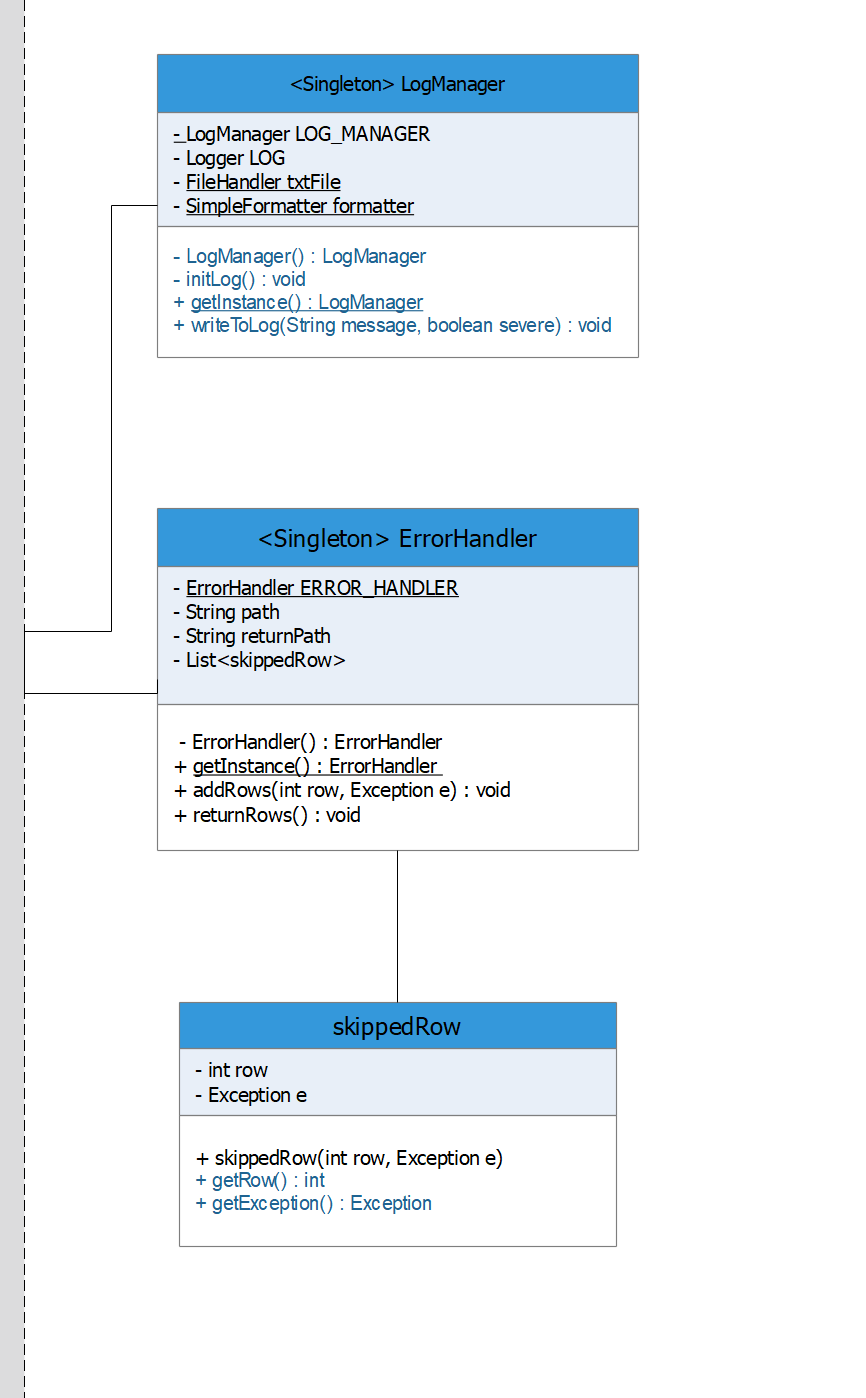
\includegraphics[scale=0.6]{uml/screenshots/errors}
\caption{Klassen für das Log- und Error-Handling}
\end{figure}
\clearpage

\subsection{skippedRow}

\paragraph{Beschreibung}
Wrapper-Klasse für übersprungene Zeilen mit zugehörigem Fehler.


\paragraph{Attribute}

\begin{enumerate}[$\bullet$]
	\item \textit{Integer row} Die Zeile
	\item \textit{Exception exception} Der aufgetretene Fehler
\end{enumerate}



\paragraph{Konstruktoren}
\begin{enumerate}[+]
	\item \textit{skippedRow(Integer row, Exception e)} \\
	Erzeugt eine neue SkippedRow-Instanz
	\begin{enumerate}[$\bullet$]
		\item \textit{Integer row:} Die Zeile in der die Exception aufgetreten ist
		\item \textit{Exception e:} Die genaue Exception, die aufgetreten ist
	\end{enumerate}	
\end{enumerate}


\clearpage
\subsection{ErrorHandler}

\paragraph{Beschreibung}
Diese Klasse nimmt Fehlermeldungen entgegen und behandelt sie (wenn möglich).


\paragraph{Methoden}

\begin{itemize}
\item + notify(String message) : void
Informiert den User über ein Ereignis, entweder durch eine Popup Message oder über das Log-Fenster (Je nach Dringlichkeit)

\item + identify(String message) : boolean
Stellt fest um welchen Fehler es sich handelt und leitet entsprechende Maßnahmen ein. (z.b Zeile überspringen)
Gibt zurück ob der Fehler behandelt werden konnte oder nicht.

\item + identify(Exception e) : boolean
Identifiziert den Exception Typ und behandelt die Exception.(I.d.r Zeile überspringen)
Gibt zurück ob die Exception behandelt werden konnte.

\item - skipRow() : void
Sort dafür, dass die aktuelle Zeile übersprungen wird.
\end{itemize}
\clearpage
\subsection{Logmanager}

\paragraph{Beschreibung}
Diese Klasse implementiert das Log-Fenster und hält es auf dem Laufenden.
Außerdem werden alle Imports in ein permanentes (seperates) Log geschrieben.


\paragraph{Attribute}

\begin{itemize}
	
\item \textit{- final static LogManager logManager}  
\\ Die einzige LogManager-Instanz 
\item \textit{- final Logger log}
\\ Java-Logger Instanz
\item \textit{- FileHandler txtFile}
\\ Text-File in die geschrieben wird
\item \textit{-  SimpleFormatter formatter}
\\ Text Formatter

\end{itemize}

\paragraph{Methoden}

\begin{itemize}
	
\item \textit{ - LogManager() : LogManager}  \\ Privater Konstruktor um mehrfache Erstellung zu unterbinden
\item \textit{ - initLog() : void} \\ Initialisiert einen Java-Logger
\item \textit{ + getLog() : Logger} \\ Gibt die Java-Logger Instanz zurück
\item \textit{ + static getInstance() : LogManager}  \\ Verweist auf den einmaligen LogManager
\item \textit{ + writeToLog(String message, boolean severe) : void} \\ Schreibt <msg> als info in das Log wenn <severe> false ist,
sonst als severe.
	
\end{itemize}
\clearpage
\subsection{File-Manager}
Die Klasse File-Management stellt die Funktionalität zum Abspeichern und Laden von Dateien zur Verfügung.

\paragraph{Methoden}

\begin{enumerate}[+]
	\item \textit{load(String path): File} Lädt die gespeicherte Datei und gibt das File zurück
	\begin{enumerate}[$\bullet$]
	\item \textit{String path:} Der Speicherpfad der Datei
	\end{enumerate}
	\begin{enumerate}[$\circ$]
		\item \textit{File:} Die geladene Datei
	\end{enumerate}

	\item \textit{save(String path, File file): Integer} Speichert ein File ab und gibt einen Integer als Statuscode zurück
	\begin{enumerate}[$\bullet$]
		\item \textit{String path}: Der Speicherpfad
		\item \textit{File file}: Die zu schreibende Datei
	\end{enumerate}
	\begin{enumerate}[$\circ$]
	\item \textit{Integer}: Der Statuscode
	\end{enumerate}
\end{enumerate}


